\documentclass[12pt]{article}
 
\usepackage[margin=1in]{geometry} 
\usepackage{amsmath,amsthm,amssymb}
\usepackage{float}
\usepackage{tikz}
\usetikzlibrary{arrows,shapes,trees} % loads some tikz extensions
 
\begin{document}
 
\title{Homework 3}
\author{Josh Klontz
CSE 802}
 
\maketitle

\begin{enumerate}
\item \textbf{Solve the following problems from Chapter 3 of the textbook: 1, 10, 17, 19}
\subitem \textbf{1. Let $x$ have an exponential density}
  \begin{equation}
    p(x|\theta) = \left\{\begin{array}{ll}\theta e^{-\theta x}&x\geq 0\\0&otherwise\end{array}\right.
  \end{equation}
  \begin{enumerate}
  \item \textbf{Plot $p(x|\theta)$ versus $x$ for $\theta = 1$. Plot $p(x|\theta)$ versus $\theta$, $(0 \leq \theta \leq 5)$, for $x=2$.}
    \begin{equation}
      p(x|1) = \left\{\begin{array}{ll} e^{-x}&x\geq 0\\0&otherwise\end{array}\right.
    \end{equation}
    \begin{figure}[H]
      \centering
      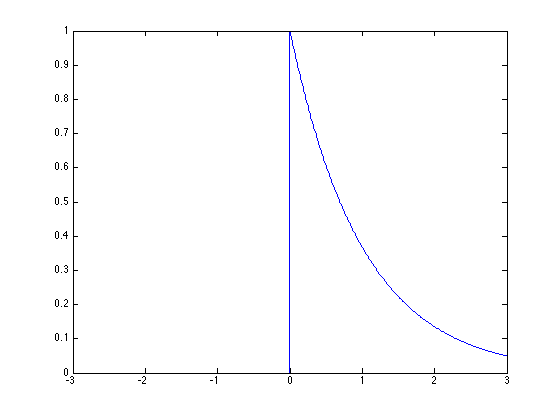
\includegraphics[width=4in]{1a1}
      \caption{$p(x|\theta)$ versus $x$ for $\theta = 1$.}
    \end{figure}
  \begin{equation}
    p(2|\theta) = \theta e^{-2\theta}
  \end{equation}
  \begin{figure}[H]
      \centering
      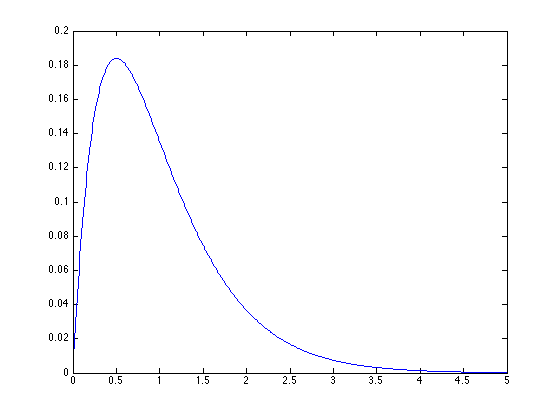
\includegraphics[width=4in]{1a2}
      \caption{$p(x|\theta)$ versus $\theta$, $(0 \leq \theta \leq 5)$, for $x=2$.}
    \end{figure}
  \item \textbf{Suppose that $n$ samples $x_1,...,x_n$ are drawn independently according to $p(x|\theta)$. Show that the maximum likelihood estimate for $\theta$ is given by}
    \begin{equation}
      \hat{\theta} = \frac{1}{\frac{1}{n}\sum_{k=1}^nx_k}
    \end{equation}
    \begin{equation}
    \begin{split}
      p(D|\theta)& = \prod_{k=1}^n p(x_k|\theta) \\
      & = \prod_{k=1}^n \left\{\begin{array}{ll}\theta e^{-\theta x_k}&x_k\geq 0\\0&otherwise\end{array}\right. \\
      & = \prod_{k=1}^n \theta e^{-\theta x_k} \\
      & = \theta^n \prod_{k=1}^n e^{-\theta x_k} \\
      & = \theta^n e^{-\theta \sum_{k=1}^n x_k} \\
      0& = ln(p(D|\theta))^\prime \\
      & = ln(\theta^n e^{-\theta \sum_{k=1}^n x_k})^\prime \\
      & = ln(\theta^n)^\prime - (\theta \sum_{k=1}^n x_k)^\prime \\
      & = \frac{n}{\theta} - \sum_{k=1}^n x_k \\
      \hat{\theta}& = \frac{n}{\sum_{k=1}^nx_k} \\
      & = \frac{1}{\frac{1}{n}\sum_{k=1}^nx_k} \\
      & \qed
    \end{split}
    \end{equation}
  \item \textbf{On your graph generated with $\theta = 1$ in part (a), mark the maximum likelihood estimate $\hat{\theta}$ for large $n$.}
    \begin{equation}
    \begin{split}
      \hat{\theta}& = \frac{1}{\frac{1}{n}\sum_{k=1}^nx_k} \\
      & \approx \frac{1}{\bar{x}} \\
      & = \frac{1}{\int_0^\infty e^{-x} dx} \\
      & = \frac{1}{-e^{-x}|_0^\infty} \\
      & = \frac{1}{-e^{-\infty} - -e^{-0}} \\
      & = \frac{1}{0 + 1} \\
      & = 1 \\
    \end{split}
    \end{equation}
    \begin{figure}[H]
      \centering
      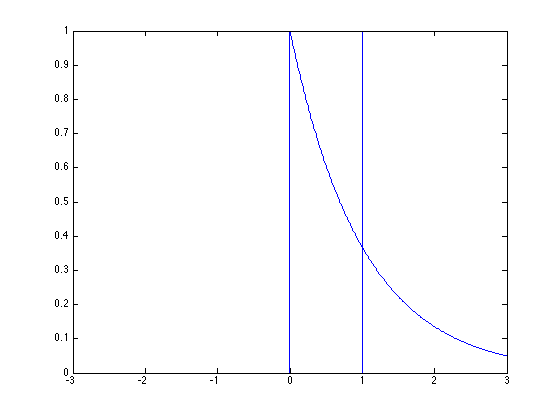
\includegraphics[width=4in]{1c}
      \caption{$p(x|\theta)$ versus $x$ for $\theta = 1$. $\hat{\theta} = 1$.}
    \end{figure}
  \end{enumerate}
  \subitem \textbf{10. Suppose we employ a novel method for estimating the mean of a data set $D = \{x_1,x_2,...,x_n\}$: We assign the mean to be the value of the first point in the set, that is, $x_1$.}
  \begin{enumerate}
  \item \textbf{Show that this method is unbiased.} \\
    The method is \emph{unbiased} if the expected value over all data sets of size $n$ is equal to the true mean.
    \begin{equation}
    \begin{split}
      D& = \{x_1,x_2,...,x_n\} \\
      \theta(D)& = x_1 \\
      E(\theta(D))& = \frac{\sum_{k=0}^{n!} \theta(permutation_k(D))}{n!} \\
      & = \frac{\sum_{i=0}^{n} x_i \cdot (n-1)!}{n \cdot (n-1)!} \\
      & = \frac{1}{n}\sum_{i=0}^{n} x_i \\
      & \qed
    \end{split}
    \end{equation}
  \item \textbf{State why this method is nevertheless highly undesirable.} \\
  This method is highly undesirable because the error of the method is equal to the variance of the data. A much more stable estimate of the mean can be computed by actually taking the average of all the data points.
  \end{enumerate}
\item \textbf{Consider a two-category classification problem with two-dimensional feature vector $X=(x_1,x_2)^T$.}
  \begin{enumerate}
  \item \textbf{Generate 300 samples from class $w_1$ and 700 samples from class $w_2$ using the \texttt{mvnrnd} function in MATLAB, and find the ML estimate of the mean vectors and covariance matrices for each of the class conditionals using the samples.}
    \begin{figure}[H]
    \begin{equation}
    \begin{split}
      \hat{u}& = \frac{1}{n}\sum_{k=1}^nx_k \\
      \hat{u1}& = [0.9141, 1.9753]^t \\
      \hat{u2}& = [1.0182, -1.9893]^t \\
      \hat{\Sigma}& = \frac{1}{n}\sum_{k=1}^n (x_k-\hat{u})(x_k-\hat{u})^t \\
      \hat{\Sigma_1}& = \left[\begin{array}{cc}2.0145 & 1.0213 \\ 1.0213 & 0.9518\end{array}\right] \\
      \hat{\Sigma_2}& = \left[\begin{array}{cc}1.0346 & 1.0471 \\ 1.0471 & 2.0379\end{array}\right] \\
    \end{split}
    \end{equation}
    \caption{Maximum Likelihood Estimations}
    \end{figure}
  \item \textbf{Find the Bayes decision boundary based on the estimated distributions and compare it with the true Bayes decision boundary by plotting the samples and the two decision boundaries in two dimensional feature space.}
    \begin{equation}
    \begin{split}
      g& = p(X|w_2)P(w_2) - p(X|w_1)P(w_1) \\
      & = 0.7\cdot|\boldsymbol{\Sigma_2}|^{1/2} \exp\left[\frac{1}{2}(\mathbf{x}-\boldsymbol{\mu_2})^t\boldsymbol{\Sigma_2}^{-1}(\mathbf{x}-\boldsymbol{\mu_2})\right] -
 0.3\cdot|\boldsymbol{\Sigma_1}|^{1/2} \exp\left[\frac{1}{2}(\mathbf{x}-\boldsymbol{\mu_1})^t\boldsymbol{\Sigma_1}^{-1}(\mathbf{x}-\boldsymbol{\mu_1})\right] \\
    \end{split}
    \end{equation}
  Didn't bother simplifying further, instead just plugged it into MATLAB.
    \begin{figure}[H]
      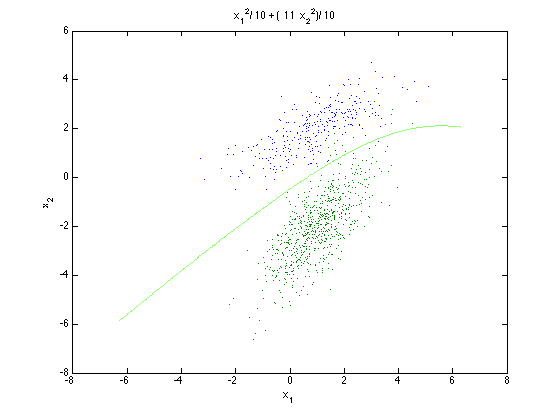
\includegraphics{2b}
      \caption{The two boundaries are indistinguishable.}
    \end{figure}
  \end{enumerate}
  \subitem \textbf{17. Let the conditional probability for a given category be given by $P(x|\theta) = \prod_{i=1}^d\theta_i^{x_i}(1-\theta_i)^{1-x_i}$.}
  \begin{enumerate}
  \item \textbf{If $s=(s_1,...,s_d)^t$ is the sum of the $n$ samples, show that $P(D|\theta)=\prod_{i=1}^d\theta_i^{s_i}(1-\theta_i)^{n-s_i}$.}
    \begin{equation}
    \begin{split}
      P(D|\theta)& =\prod_{k=1}^nP(x_k|\theta) \\
      & = \prod_{k=1}^n\prod_{i=1}^d\theta_i^{x_{ki}}(1-\theta_i)^{1-x_{ki}} \\
      & = \prod_{i=1}^d\prod_{k=1}^n\theta_i^{x_{ki}}(1-\theta_i)^{1-x_{ki}} \\
      & = \prod_{i=1}^d(\theta_i^{x_{1i}}\cdot\theta_i^{x_{2i}}\cdots\theta_i^{x_{ni}})((1-\theta_i)^{1-x_{1i}}\cdot(1-\theta_i)^{1-x_{2i}}\cdots(1-\theta_i)^{1-x_{ni}}) \\
      & = \prod_{i=1}^d\theta_i^{\sum_{k=1}^nx_{ki}}(1-\theta_i)^{\sum_{k=1}^n1-x_{ki}} \\
      & = \prod_{i=1}^d\theta_i^{\sum_{k=1}^nx_{ki}}(1-\theta_i)^{n-\sum_{k=1}^nx_{ki}} \\
      & =\prod_{i=1}^d\theta_i^{s_i}(1-\theta_i)^{n-s_i} \\
      & \qed
    \end{split}
    \end{equation}
  \item \textbf{Assuming a uniform prior distribution for $\theta$ show that $p(\theta|D)=\prod_{i=1}^d\frac{(n+1)!}{s_i!(n-s_i)!}\theta_i^{s_i}(1-\theta_i)^{n-s_i}$.}
    \begin{equation}
    \begin{split}
      p(\theta|D)& = \frac{p(D|\theta)p(\theta)}{\int p(D|\theta)p(\theta)d\theta} \\
      & = \frac{p(D|\theta)}{\int p(D|\theta)d\theta} \\
      & = \frac{\prod_{i=1}^d\theta_i^{s_i}(1-\theta_i)^{n-s_i}}{\int \prod_{i=1}^d\theta_i^{s_i}(1-\theta_i)^{n-s_i}d\theta} \\
      & = \prod_{i=1}^d\frac{1}{\int \theta_i^{s_i}(1-\theta_i)^{n-s_i}d\theta}\theta_i^{s_i}(1-\theta_i)^{n-s_i} \\
      & = \prod_{i=1}^d\frac{1}{\frac{s_1!(n-s_i)!}{(s_i+(n-s_i)+1)!}}\theta_i^{s_i}(1-\theta_i)^{n-s_i} \\
      & = \prod_{i=1}^d\frac{(n+1)!}{s_i!(n-s_i)!}\theta_i^{s_i}(1-\theta_i)^{n-s_i} \\
      & \qed
    \end{split}
    \end{equation}
  \item \textbf{Plot this density for the case $d=1, n=1$ and for the two resulting possibilities for $s1$.}
    \begin{equation}
    \begin{split}
      p(\theta|D)& =\prod_{i=1}^d\frac{(n+1)!}{s_i!(n-s_i)!}\theta_i^{s_i}(1-\theta_i)^{n-s_i} \\
      & =\frac{(1+1)!}{s_1!(1-s_1)!}\theta_1^{s_1}(1-\theta_1)^{1-s_1} \\
      & =\frac{2}{s_1!(1-s_1)!}\theta^{s_1}(1-\theta)^{1-s_1} \\
      p(\theta|s_i=0)& =2(1-\theta) \\
      p(\theta|s_i=1)& =2\theta \\
    \end{split}
    \end{equation}
    \begin{figure}[H]
      \centering
      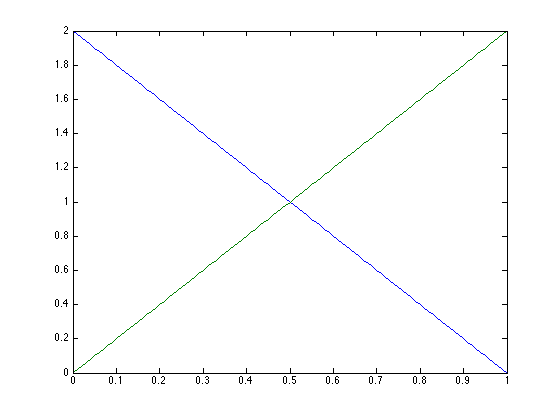
\includegraphics[width=4in]{17c}
      \caption{$p(\theta|s_i=0) = blue, p(\theta|s_i=1) = green$}
    \end{figure}
  \item \textbf{Integrate the product $P(x|\theta)p(\theta|D)$ over $\theta$ to obtain the desired conditional probability $P(x|D)=\prod_{i=1}^d(\frac{s_i+1}{n+2})^{x_1}(1-\frac{s_i+1}{n+2})^{1-x_i}$.}
    \begin{equation}
    \begin{split}
      & =\int P(x|\theta)p(\theta|D) d\theta \\
      & =\int \prod_{i=1}^d\theta_i^{x_i}(1-\theta_i)^{1-x_i}\prod_{i=1}^d\frac{(n+1)!}{s_i!(n-s_i)!}\theta_i^{s_i}(1-\theta_i)^{n-s_i} d\theta \\
      & =\prod_{i=1}^d\frac{(n+1)!}{s_i!(n-s_i)!} \cdot \int \prod_{i=1}^d\theta_i^{x_i}(1-\theta_i)^{1-x_i}\theta_i^{s_i}(1-\theta_i)^{n-s_i} d\theta \\
      & =\prod_{i=1}^d\frac{(n+1)!}{s_i!(n-s_i)!} \cdot \prod_{i=1}^d \int \theta_i^{s_i+x_i}(1-\theta_i)^{n-s_i+1-x_i} d\theta \\
      & =\prod_{i=1}^d\frac{(n+1)!}{s_i!(n-s_i)!} \cdot \prod_{i=1}^d \frac{(s_i+x_i)!(n-s_i+1-x_i)!}{(s_i+x_i+n-s_i+1-x_i+1)!} \\
      & =\prod_{i=1}^d\frac{(n+1)!(s_i+x_i)!(n-s_i+1-x_i)!}{s_i!(n-s_i)!(n+2)!} \\
      & =\prod_{i=1}^d\frac{(s_i+x_i)!(n-s_i+1-x_i)!}{s_i!(n-s_i)!(n+2)} \\
      & = ...\ (Not\ sure)\\
      & =\prod_{i=1}^d(\frac{s_i+1}{n+2})^{x_1}(1-\frac{s_i+1}{n+2})^{1-x_i}
    \end{split}
    \end{equation}
  \item \textbf{If we think of obtaining $P(x|D)$ by substituting an estimate $\hat{\theta}$ or $\theta$ in $P(x|\theta)$, what is the effective Bayesian estimate for $\theta$?} \\
    An effective Bayesian estimate for $\theta$ is 0.5 because it maximizes $p(\theta|D)$.
  \end{enumerate}
\subitem \textbf{19. Assume we have training data from a Gaussian distribution of known covariance $\Sigma$ but unknown mean $\mu$. Suppose further that this mean itself is random, and characterized by a Gaussian density having mean $\mu_0$ and covariance $\Sigma_0$.}
  \begin{enumerate}
  \item \textbf{What is the MAP estimator for $\mu$?} \\
    The MAP estimator for $\mu$ is the mode of its Gaussian density, $\mu_0$.
  \item \textbf{Suppose we transform our coordinates by a linear transform $x^\prime=Ax$, for non-singular matrix A, and accordingly for other terms. Determine whether your MAP esimator gives the appropriate estimate for the transformed mean $\mu^\prime$. Explain.} \\
    The MAP estimator gives the appropriate estimate for the transformed mean $\mu^\prime = A\mu_0$ because the mode of a linear transform of a distribution is the linear transform of the distrubution's mode.
  \end{enumerate}
\item \textbf{Consider data uniformly distributed in a d-dimensional unit hypersphere. The neighborhood of a point $x$ is defined as a hypersphere of radius $l$ around $x$. A neighborhood is called $significant$ if it captures a fraction $r$ of the total volume of the unit hypersphere. Write the expression for the significant neighborhood $l$ of a point $x$, assuming $x$ and its neighborhood lie completely within the unit hypersphere. How large should $l$ be to capture 25\% of the data $(r = 0.25)$ when the dimensionality varies as $d = 1, 2, 5, 10, 50, 100, 500, 1000$? What can one infer by observing the size of the significant neighborhood as a function of $d$?}
  \begin{figure}[H]
    \begin{equation}
      V_d = \frac{\pi^\frac{d}{2}}{\Gamma(\frac{d}{2}+1)}R^d
    \end{equation}
    \caption{Volume of an d-dimensional hypersphere.}
  \end{figure}
  \begin{figure}[H]
    \begin{equation}
    \begin{split}
      r& = \frac{\frac{\pi^\frac{d}{2}}{\Gamma(\frac{d}{2}+1)}l^d}{\frac{\pi^\frac{d}{2}}{\Gamma(\frac{d}{2}+1)}1^d} \\
      r& = l^d \\
      l& = r^\frac{1}{d}
    \end{split}
    \end{equation}
    \caption{The significant neighborhood $l$ of a point $x$.}
  \begin{table}[H]
    \centering
    \begin{tabular}{ll}
      $d$ & $l$ \\ \hline
      1 & 0.25 \\
      2 & 0.5 \\
      5 & 0.75785828325 \\
      10 & 0.87055056329 \\
      50 & 0.97265494741 \\
      100 & 0.98623270449 \\
      500 & 0.99723125135 \\
      1000 & 0.9986146661 \\
    \end{tabular}
    \caption{How large $l$ should be when $r=0.25$.}
    \end{table}
  \end{figure}
  The size of the significant neighborhood increases as a function of $d$ and approaches $\infty$ when $d \rightarrow \infty$.
\end{enumerate}

\end{document}
